\documentclass[tikz,border=8pt]{standalone}
% Shared look for every TikZ diagram. Load with % Shared look for every TikZ diagram. Load with % Shared look for every TikZ diagram. Load with \input{../../tools/tikz-style.tex}
\usepackage[T1]{fontenc}
\usepackage{lmodern}
\renewcommand{\sfdefault}{lmr}  % diagrams use the same serif as the text
\usetikzlibrary{arrows.meta, positioning, shapes.geometric, calc, fit, backgrounds}
\definecolor{cblue}{HTML}{4C78A8}
\definecolor{corange}{HTML}{F58518}
\definecolor{cgreen}{HTML}{54A24B}
\definecolor{cred}{HTML}{E45756}
\definecolor{cpurple}{HTML}{B279A2}
\definecolor{cgrey}{HTML}{6B6B6B}
\tikzset{
  every picture/.style={font=\sffamily, line width=1.2pt},
  box/.style={draw=#1, fill=#1!12, rounded corners=4pt, align=center, inner sep=7pt, minimum height=1.1cm},
  box/.default=cgrey,
  arrow/.style={-{Stealth[length=3mm]}, draw=cgrey, line width=1.4pt},
  title/.style={font=\sffamily\bfseries\Large},
  note/.style={font=\sffamily\small, text=cgrey, align=center},
}
\AtBeginDocument{\hyphenpenalty=10000 \exhyphenpenalty=10000}

\usepackage[T1]{fontenc}
\usepackage{lmodern}
\renewcommand{\sfdefault}{lmr}  % diagrams use the same serif as the text
\usetikzlibrary{arrows.meta, positioning, shapes.geometric, calc, fit, backgrounds}
\definecolor{cblue}{HTML}{4C78A8}
\definecolor{corange}{HTML}{F58518}
\definecolor{cgreen}{HTML}{54A24B}
\definecolor{cred}{HTML}{E45756}
\definecolor{cpurple}{HTML}{B279A2}
\definecolor{cgrey}{HTML}{6B6B6B}
\tikzset{
  every picture/.style={font=\sffamily, line width=1.2pt},
  box/.style={draw=#1, fill=#1!12, rounded corners=4pt, align=center, inner sep=7pt, minimum height=1.1cm},
  box/.default=cgrey,
  arrow/.style={-{Stealth[length=3mm]}, draw=cgrey, line width=1.4pt},
  title/.style={font=\sffamily\bfseries\Large},
  note/.style={font=\sffamily\small, text=cgrey, align=center},
}
\AtBeginDocument{\hyphenpenalty=10000 \exhyphenpenalty=10000}

\usepackage[T1]{fontenc}
\usepackage{lmodern}
\renewcommand{\sfdefault}{lmr}  % diagrams use the same serif as the text
\usetikzlibrary{arrows.meta, positioning, shapes.geometric, calc, fit, backgrounds}
\definecolor{cblue}{HTML}{4C78A8}
\definecolor{corange}{HTML}{F58518}
\definecolor{cgreen}{HTML}{54A24B}
\definecolor{cred}{HTML}{E45756}
\definecolor{cpurple}{HTML}{B279A2}
\definecolor{cgrey}{HTML}{6B6B6B}
\tikzset{
  every picture/.style={font=\sffamily, line width=1.2pt},
  box/.style={draw=#1, fill=#1!12, rounded corners=4pt, align=center, inner sep=7pt, minimum height=1.1cm},
  box/.default=cgrey,
  arrow/.style={-{Stealth[length=3mm]}, draw=cgrey, line width=1.4pt},
  title/.style={font=\sffamily\bfseries\Large},
  note/.style={font=\sffamily\small, text=cgrey, align=center},
}
\AtBeginDocument{\hyphenpenalty=10000 \exhyphenpenalty=10000}

% The three equations of Luong attention and of self-attention side by side. Colours mark what replaces what:
% query (blue), key (orange), value (green); everything else is identical.
\newcommand{\Q}[1]{\textcolor{cblue}{\boldsymbol{#1}}}
\newcommand{\K}[1]{\textcolor{corange}{\boldsymbol{#1}}}
\newcommand{\V}[1]{\textcolor{cgreen}{\boldsymbol{#1}}}
\begin{document}
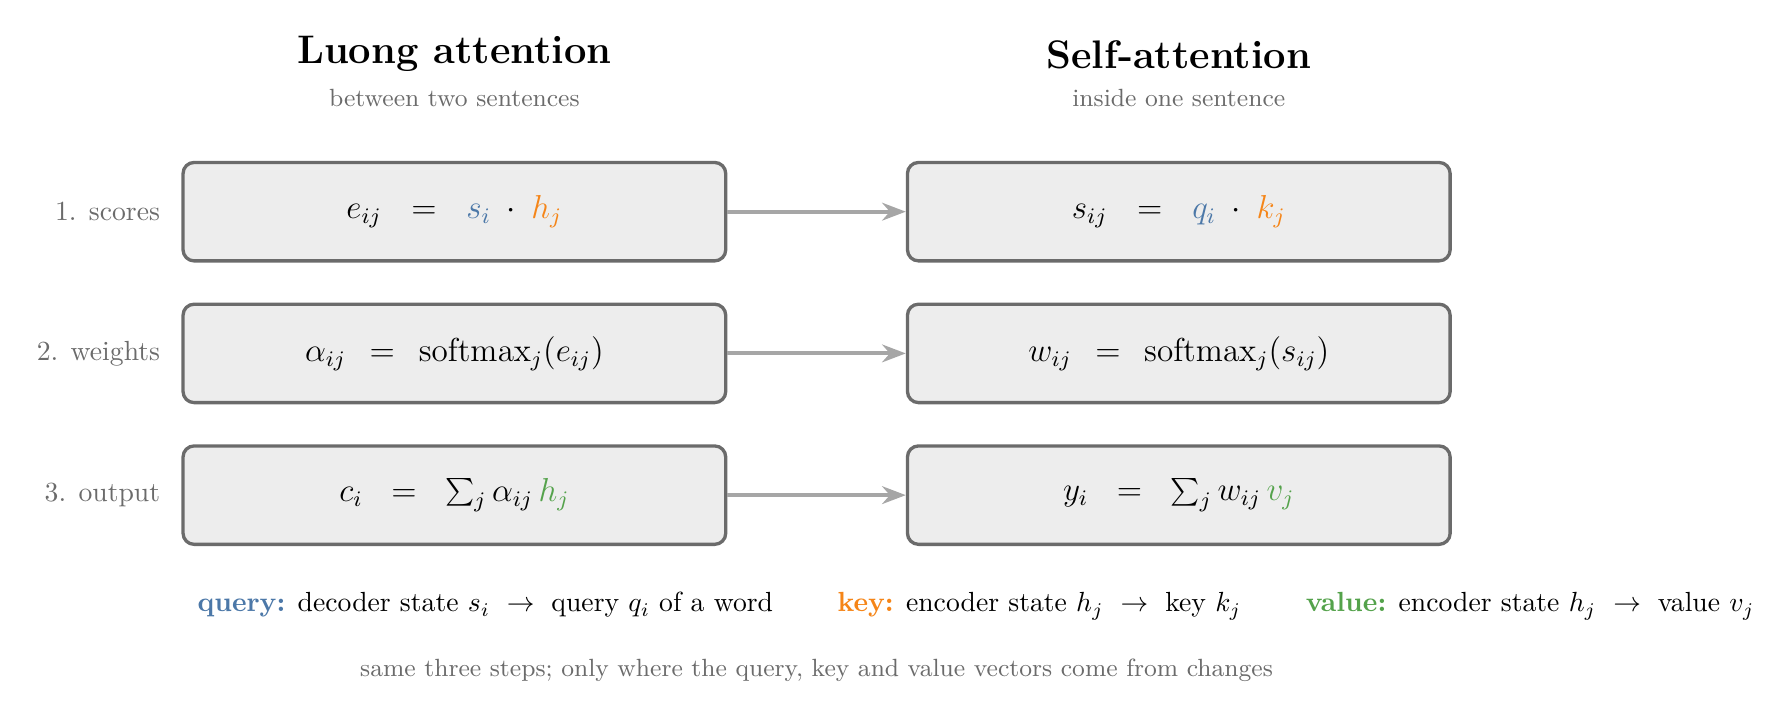
\begin{tikzpicture}[eq/.style={box=cgrey, text width=6.4cm, minimum height=1.25cm, font=\large},
  head/.style={font=\sffamily\bfseries\Large}, stp/.style={font=\sffamily, text=cgrey, align=right, anchor=east}]
  \node[head] at (0, 1.4) {Luong attention};
  \node[head] at (9.2, 1.4) {Self-attention};
  \node[font=\sffamily\small, text=cgrey] at (0, 0.85) {between two sentences};
  \node[font=\sffamily\small, text=cgrey] at (9.2, 0.85) {inside one sentence};
  \foreach \y/\name/\l/\r in {
      0/{1. scores}/{$e_{ij} = \Q{s_i} \cdot \K{h_j}$}/{$s_{ij} = \Q{q_i} \cdot \K{k_j}$},
      -1.8/{2. weights}/{$\alpha_{ij} = \mathrm{softmax}_j(e_{ij})$}/{$w_{ij} = \mathrm{softmax}_j(s_{ij})$},
      -3.6/{3. output}/{$c_i = \sum_j \alpha_{ij}\,\V{h_j}$}/{$y_i = \sum_j w_{ij}\,\V{v_j}$}} {
    \node[eq] (L) at (0, \y-0.6) {\l};
    \node[eq] (R) at (9.2, \y-0.6) {\r};
    \node[stp] at (-3.6, \y-0.6) {\name};
    \draw[arrow, draw=cgrey!60] (L.east) -- (R.west);
  }
  \node[align=left, font=\sffamily, anchor=north west] at (-3.4, -5.3) {
    \textcolor{cblue}{\textbf{query:}} decoder state $s_i$ \;$\to$\; query $q_i$ of a word \qquad
    \textcolor{corange}{\textbf{key:}} encoder state $h_j$ \;$\to$\; key $k_j$ \qquad
    \textcolor{cgreen}{\textbf{value:}} encoder state $h_j$ \;$\to$\; value $v_j$};
  \node[note, anchor=north] at (4.6, -6.15) {same three steps; only where the query, key and value vectors come from changes};
\end{tikzpicture}
\end{document}
